% !TEX encoding = UTF-8 Unicode
\documentclass[a4paper]{article}

\usepackage[utf8]{inputenc}
\usepackage{erk}
\usepackage{times}
\usepackage{graphicx}
\usepackage{xcolor}
\usepackage[top=22.5mm, bottom=22.5mm, left=22.5mm, right=22.5mm]{geometry}

\usepackage[slovene,english]{babel}

\newcommand\todocomment[1]{\textcolor{red}{||TODO:\\ #1\\||}}


% local definitions
\def\footnotemark{}%  to avoid footnote on cover page

\begin{document}
%make title
\title{Utilizing Convolution for Obstacle Avoidance during Robotic Manipulator Movement}

\author{Jakob Baumgartner$^{1}$, Gregor Klančar$^{2}$} % use ^1, ^2 for author(s) from different institutions

\affiliation{$^{1}$Fakulteta za Elektrotehniko, Tržaška cesta 25, 1000 Ljubljana\\}

\email{E-pošta: jakob.baumgartner@fe.uni-lj.si}

\maketitle

%\thispagestyle{empty}

\begin{abstract}{Abstract}
For the papers written in Slovene language an English title and abstract is required. The abstract should be no more than 200 words. 

We accept only electronic submissions in pdf (without password protection) or Microsoft Word format. Submission form can be found on ERK web page \cite{ERK}.
\end{abstract}


\selectlanguage{slovene}

\section{Introduction }

Robotic manipulators, specifically those with a high degree of freedom (DOF), possess a crucial characteristic known as kinematic redundancy. Kinematic redundancy refers to having more joints (i.e., degrees of freedom - DOF) than required to perform a task, thus allowing the robot to adopt multiple configurations to accomplish the same end-effector position and orientation. This redundancy provides a considerable advantage, making it possible for manipulators to optimize movement according to different criteria, such as energy efficiency, obstacle avoidance, or joint limit avoidance.

In this research, we specifically consider a 7-DOF Panda Emika manipulator. When controlling both the position and orientation of the end-effector in a 3D space, which requires six degrees of freedom (three for position and three for orientation), a 7-DOF manipulator such as the Panda Emika has one redundant degree. However, when controlling only the position, which requires three degrees of freedom, the manipulator possesses four redundant degrees. This redundancy grants the manipulator an essential characteristic: an infinite number of possible joint configurations to reach a specific end-effector (EE) point in space.

When dealing with redundant manipulators, task prioritization is crucial. In our approach, we distinguish between primary and secondary tasks. The primary task of the manipulator is usually defined as reaching a desired EE position and orientation or as following a trajectory made out of such points. In this work we instead use APF (Artificial Potential Field), to guide the EE towards the goal position, while avoiding the obstacles in the path of the EE. Operating in a real-world environment often requires considering secondary tasks, such as real-time obstacle avoidance, to ensure safe and uninterrupted operation of the manipulator.

This paper proposes a novel method for real-time obstacle avoidance in the Panda Emika 7-DOF manipulator. We use an obstacle grid combined with convolution techniques to assign avoidance directions to each manipulator segment, ensuring efficient and safe maneuvering within complex environments. 

\todocomment{Dodaj opis poglavij.}

\section{Background and Related Work}

The execution of the secondary task of obstacle avoidance necessitates an understanding of the spatial relationship between the manipulator and surrounding obstacles, usually quantified as a distance or interpreted as a repulsive force. By conceptualizing obstacles as sources of repulsive forces, the manipulator can be guided away from potential collisions, akin to how two magnets of the same polarity repel each other.

Two commonly employed methods for obstacle avoidance include potential field methods and artificial neural networks. In potential field methods, the robot and obstacles are treated as charged entities. The robot is attracted to the target (goal) while being repelled by obstacles, resulting in a potential field. The robot navigates this field, moving along the path of steepest descent. While this method is intuitive and relatively easy to implement, it can sometimes result in local minima problems where the robot gets stuck in a position that is not the target but cannot find a path due to the repelling obstacles.

Artificial neural networks (ANNs) are another prevalent approach, offering potential solutions to the local minima problem. By learning to map sensor readings to appropriate actions, ANNs can be trained to successfully navigate complex environments. However, they require extensive training and can be computically intensive.

Our proposed approach seeks to combine the strengths of these methods, utilizing the obstacle grid and convolution techniques to efficiently calculate repulsive forces, thus enabling real-time obstacle avoidance while mitigating issues commonly associated with traditional methods.

\todocomment{Preveri pravilnost informacij, dodaj vire, ki potrjujejo informacije.}

\todocomment{preveri podobnost naše metode z metodo: Vector Field Histogram (VFH) }

\section{Methodology }

\subsection{Obstacle Grid}

\subsection{Attractive Field}

APF for EE task.

\subsection{Convolution Techniques}

Sobel-like directional kernels.

\subsection{Robot Segments Control}

Null space.

\section{Experiment and Results}

The wall visualization.

Line field strenght dx,dy,dz

\section{Pisanje prispevka}

Pri pisanju uporabljajte sloge, ki so definirani v datoteki erk.sty in ne spreminjajte velikosti ali sloga pisave. Ta dokument lahko vzamete kot vzorec za oblikovanje prispevka v orodju \LaTeX.
Tabela \ref{tab1} povzema osnovne sloge in velikosti pisave.

\begin{table}[h]
\caption{Osnovni slogi pri oblikovanju prispevka.} \label{tab1}
\smallskip
\begin{center}
\begin{tabular}{ | r | c | c | }
\hline  
  \textbf{Text Style} & \textbf{Font Size} & \textbf{Attributes}\\ 
\hline  
  Paper title & 17pt & bold\\
  Author names & 12pt & bold\\
  Affiliation & 10pt & italic\\
  Heading & 12pt & bold \\
  Subheading & 10pt & bold\\
  Regular text & 10pt &\\
  Captions \& ref. & 9pt &\\
\hline  
\end{tabular}
\end{center}
\end{table}

\subsection{Enačbe in slike}

Enačbe in formule se pišejo s poševnimi črkami in so zaporedno oštevilčene. V besedilu naj bodo reference na enačbe zapisane v oklepajih (\ref{eq1}).

\begin{equation}
 \int^{r_{2}}_{0}F(r,\varphi)\; dr\; d\varphi= [\sigma r_{2} / (2\mu_{0})]
    \label{eq1}
\end{equation}

Prispevki za ERK se ne tiskajo v barvah, zato pripravite črno-bele slike. Slike naj bodo postavljene v okvirje širine enega ali dveh stolpcev in označene s številko in podnapisom. V besedilu morajo biti reference na slike (slika \ref{slika}).

\begin{figure}[!htb]
    \begin{center}
        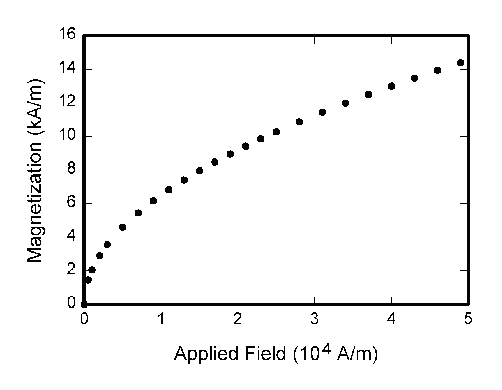
\includegraphics[scale=1]{field1.eps}
        \caption{Podajte kratko razlago slike.} \label{slika}
    \end{center}
\end{figure}

\section{Oddaja prispevka}

Prispevek oddajte v elektronski obliki preko formularja na spletni strani \cite{ERK}. Sprejemamo prispevke v formatu pdf (brez nastavljenih zaščitnih gesel) ali Microsoft Word. Pred oddajo prispevka prosimo preverite dodatne informacije za avtorje, ki so na spletnih straneh. 

Formular za elektronsko oddajo prispevkov bo aktiviran v juniju, rok za oddajo je \textbf{13. julij 2014}. Avtorje bomo obvestili o izboru konec avgusta.

\small
\begin{thebibliography}{1}

\bibitem{ERK} ERK, http://www.ieee.si/erk/index.html 
\bibitem{Zbornik} B. Zajc, A. Trost: Zbornik triindvajsete mednarodne Elektrotehniške in računalniške konference ERK 2014, 22. - 24. September 2014, Portorož, Slovenija

\end{thebibliography}

\end{document}
